\section{Architecture générale}

La figure~\ref{modele_restreint} met en évidence le sous ensemble que nous avons choisi d'étudier, qui a été déterminé à partir des contraintes énumérées au chapitre~\ref{chapter:les_contraintes}. Cette sous partie correspond à ce que Laborit nomme le néocortex.

\begin{figure}[H] 
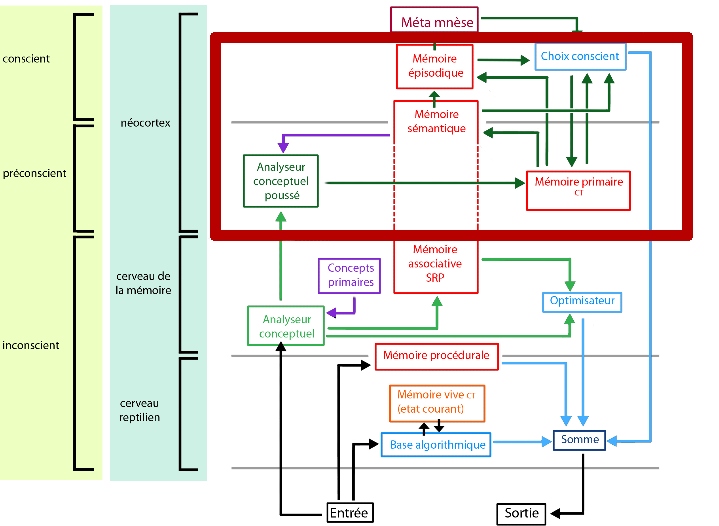
\includegraphics[width=\textwidth]{files/modele_restreint} 
\caption{Modèle restreint} 
\label{modele_restreint}
\end{figure}

\begin{figure}[H] 
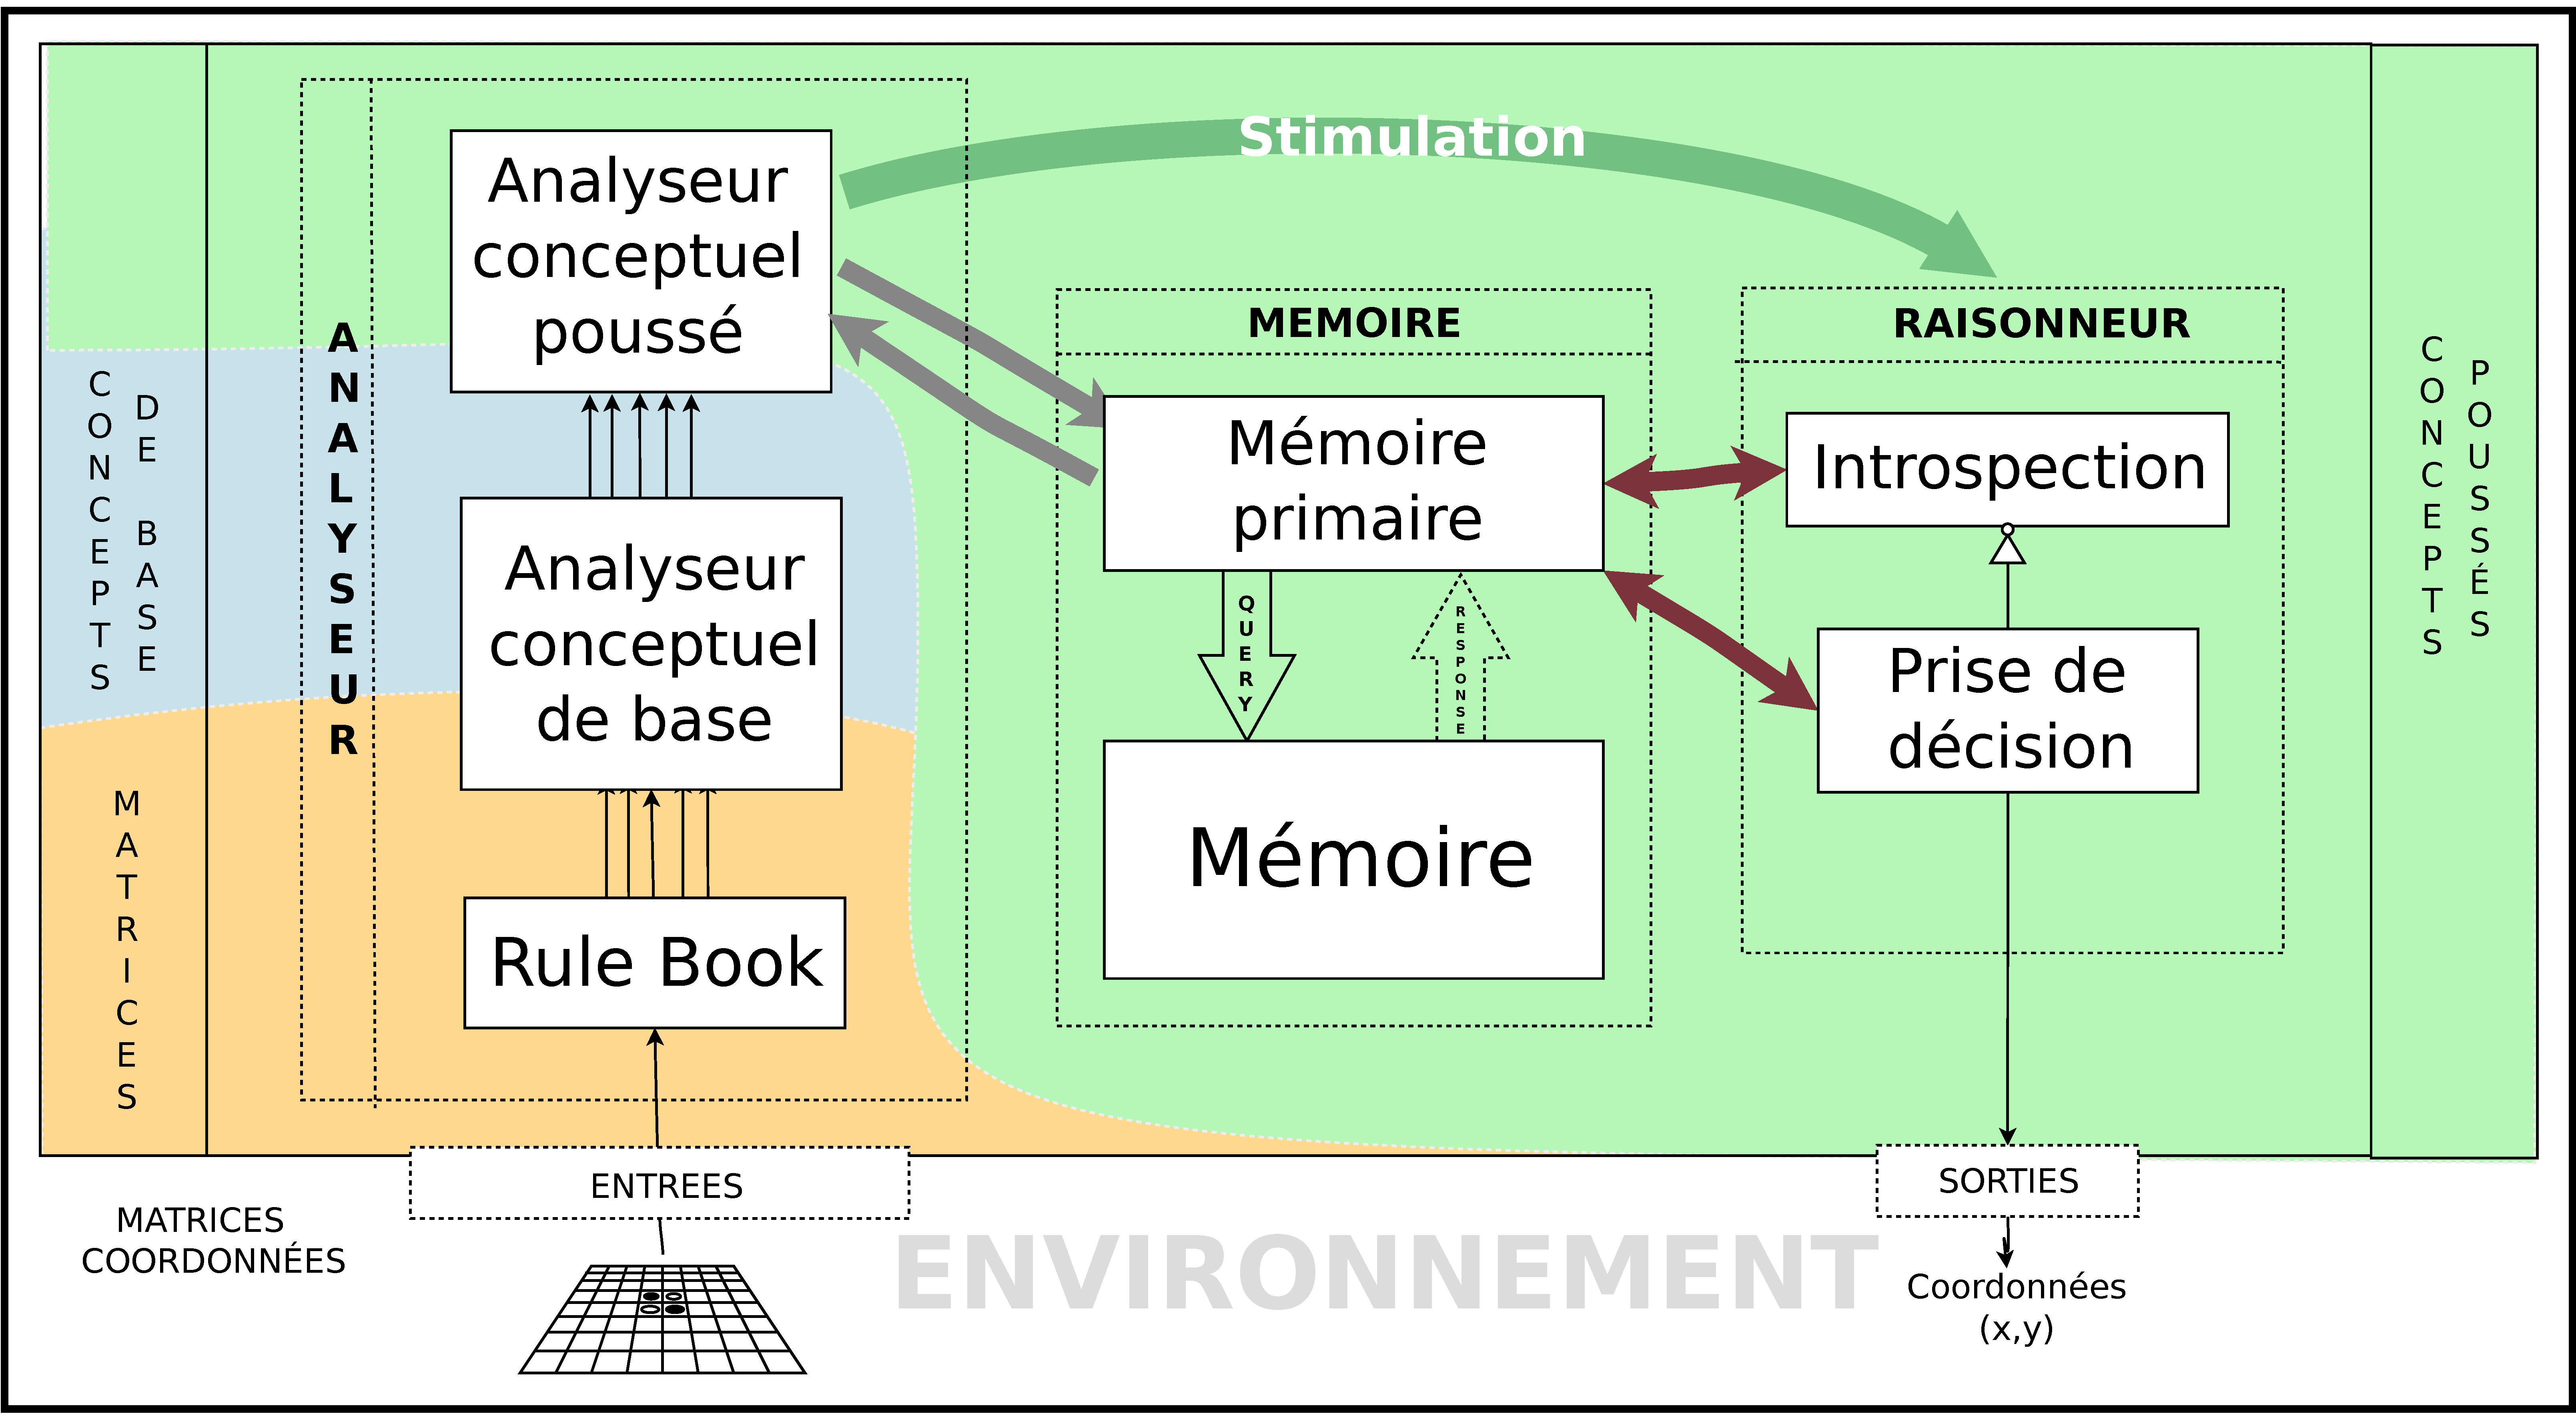
\includegraphics[width=\textwidth]{files/simplified_general_diagram} 
\caption{Schéma général} 
\label{schema_general}
\end{figure}

Nous pouvons représenter notre architecture par le schéma \ref{schema_general}. Sur ce schéma, nous pouvons voir que le plateau entre dans notre IA sous forme matricielle. Dans une première étape le \og rule book \fg{} génère un ensemble de plateau à partir des coups possibles. Cette ensemble est fourni à l'analyseur conceptuel de base qui le traduit dans un formalisme logique puis l'analyseur conceptuel poussé associe à chaque plateau un ensemble de formes reconnaissables sur ces plateaux. Le tout est ensuite transmis à la mémoire et le raisonneur et stimulé afin de déclencher la prise de décision. Celui-ci, le raisonneur, effectue une comparaison des plateaux possibles à partir des formes reconnues et une fois sa décision prise la retourne à l'environnement.
